\documentclass{scrartcl}
\usepackage[utf8]{inputenc}
\usepackage{graphicx}
\usepackage{subcaption}
\usepackage{listings}
\usepackage{color}

\definecolor{dkgreen}{rgb}{0,0.6,0}
\definecolor{gray}{rgb}{0.5,0.5,0.5}
\definecolor{mauve}{rgb}{0.58,0,0.82}

\lstset{frame=tb,
  language=Java,
  aboveskip=3mm,
  belowskip=3mm,
  showstringspaces=false,
  columns=flexible,
  basicstyle={\small\ttfamily},
  numbers=none,
  numberstyle=\tiny\color{gray},
  keywordstyle=\color{blue},
  commentstyle=\color{dkgreen},
  stringstyle=\color{mauve},
  breaklines=true,
  breakatwhitespace=true,
  tabsize=3
}



\graphicspath{ {image/} }

\title{CMPE 434 - Introduction to Robotics}
\subtitle{Lab 2: Moving to Python}
\date{Deadline: September 23, 2019}

\begin{document}
\maketitle

The aim of this lab is to:
\begin{enumerate}
    \item Get acquainted with the infrastructure that will run on your EV3 bricks,
    \item Set up the programming environment on your computers,
    \item Test out our first programs on EV3 hardware.
\end{enumerate} 

\textit{EV3 Robotics Kit} comes with a brick which essentially is a small computer. Just like Windows on your PCs or iOS on your iPhones, we need to run an operating system (OS) on this computer. \textbf{ev3dev} is the name of the OS that we are going to use for this purpose. It is a \textit{Linux-based} operating system that is specifically modified to handle EV3 hardware.
\\

\begin{figure}[h!]
    \begin{center}
        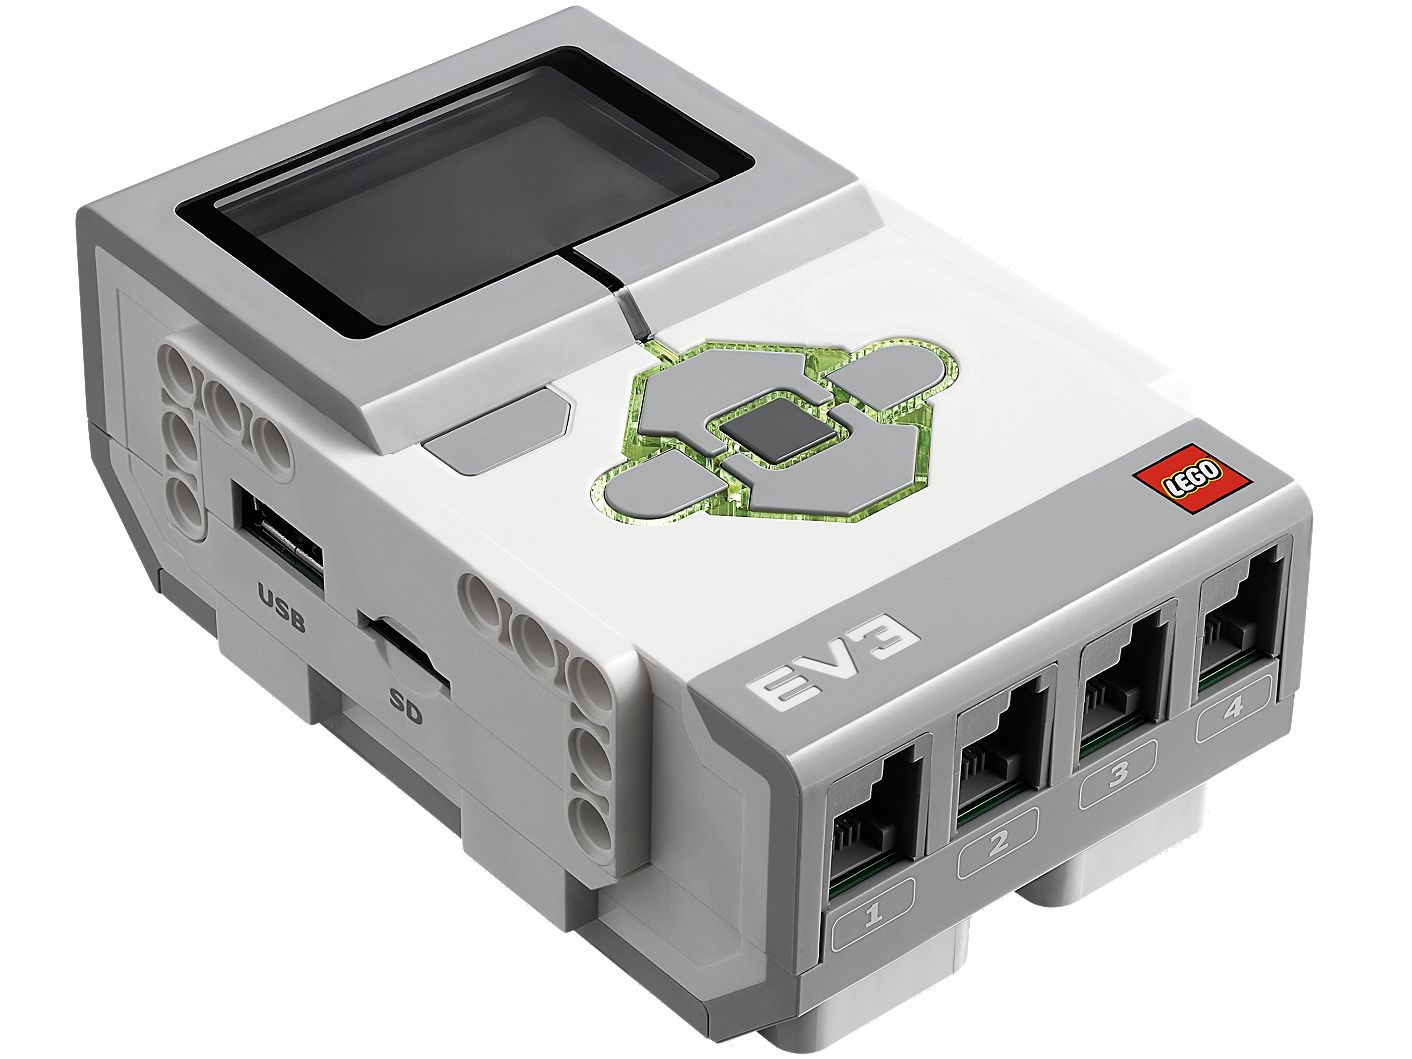
\includegraphics[width=0.5\textwidth]{brick.jpg}
        \caption{EV3 Brick}
    \end{center}
\end{figure}

By following the list below, you are expected to install \textit{ev3dev} to an SD Card and boot your brick via this medium. Then, you are asked to set up the programming environment and implement your first programs as explained below.

\newpage
\underline{Things to do:}
\begin{enumerate}
    \item Follow the instructions at this page:\\ https://www.ev3dev.org/docs/getting-started/
    \begin{itemize}
        \item Download ev3dev-stretch image
        \item If you don't have one, download and install an image-burner to write the image into the sd card. Etcher is a free tool that you can use for this purpose https://etcher.io/
        \item Burn the image of the OS to your sd card.
        \item Boot ev3dev to see the result. In the figure below, a screenshot of a successful installation is given:
        \begin{figure}[h!]
            \begin{center}
              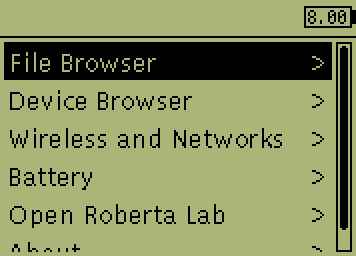
\includegraphics[width=0.3\textwidth]{main-menu.png}
              \caption{ev3dev Main menu}
            \end{center}
        \end{figure}
    \end{itemize}
    \item Install the latest version of Python: https://www.python.org/downloads/
    \item To implement Python programs and run them on the brick, download and install Visual Studio Code (VS Code): https://code.visualstudio.com/
    \item Create your workspace, a folder to be used as the container of all your programs. Under that folder, create another one, name it \textit{lab2}.
    \item Open VS Code, install \textit{Python}, \textit{ev3dev-browser} and \textit{EV3 MicroPython} extensions.
        \begin{figure}[h!]
            \begin{center}
              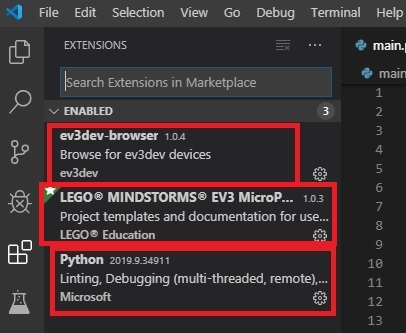
\includegraphics[width=0.3\textwidth]{ext.jpg}
              \caption{VS Code extensions}
            \end{center}
        \end{figure}
    \item After reloading, switch from \textit{Extensions} view to \textit{LEGO MINDSTORMS EV3 MicroPython} view using the menu buttons on the left. Create a new project in \textit{lab2} folder.
        \begin{figure}[h!]
            \begin{center}
              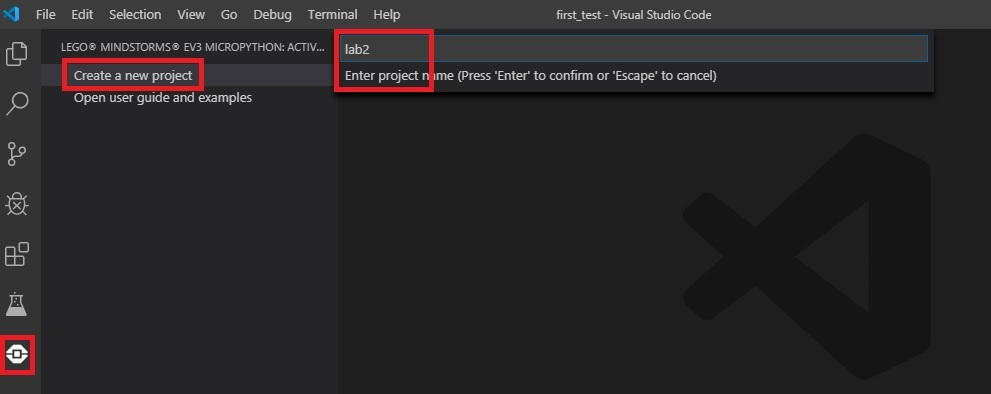
\includegraphics[width=0.75\textwidth]{new.jpg}
              \caption{Creating a new project}
            \end{center}
        \end{figure}
    \begin{itemize}
        \item You will be given a template with \textit{main.py} in it. However, we are \textbf{not} going to use this file. 
        \item Create another file for your first program, call it \textit{hello\_world.py}.
    \end{itemize}

    \item Copy and paste the following code:
        \begin{lstlisting}
            #!/usr/bin/env python3

            from ev3dev.ev3 import *
            from time import sleep
            
            Sound.speak('Hello, I am E V 3!').wait()
            lcd = Screen()
            i=0
            
            while i<50:
                lcd.clear()
                lcd.draw.text((20+i, 20+i), 'CMPE 434')
                lcd.update()
                sleep(0.05)
                i+=1
        \end{lstlisting}
    \newpage
    \item To run your code on the device, update the configuration file as shown below:
        \begin{figure}[h!]
            \begin{center}
              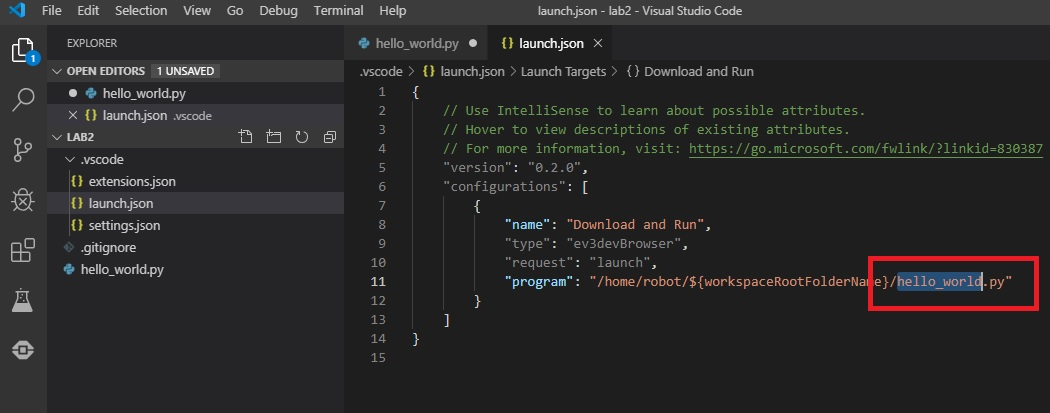
\includegraphics[width=0.75\textwidth]{cfg.jpg}
              \caption{Configuration}
            \end{center}
        \end{figure}

    \item Check if you can successfully connect to device form VS Code.
        \begin{itemize}
            \item Connect via USB.
            \item Make sure that the brick is already started.
            \item On \textit{EV3 Device Browser} menu, connect to the brick as shown.
                \begin{figure}
                    \centering
                    \begin{subfigure}{.5\textwidth}
                      \centering
                      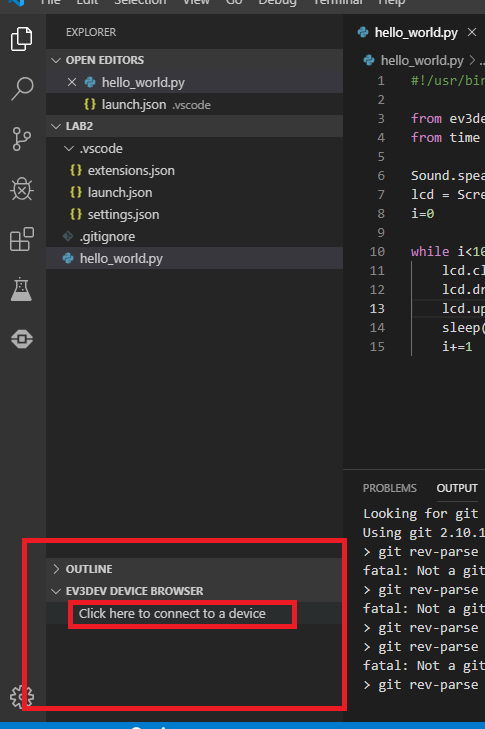
\includegraphics[width=.5\linewidth]{1.jpg}
                    \end{subfigure}%
                    \begin{subfigure}{.5\textwidth}
                      \centering
                      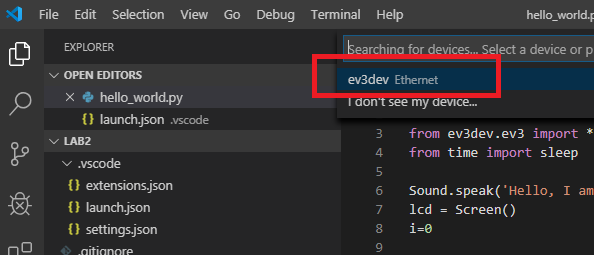
\includegraphics[width=.85\linewidth]{2.jpg}
                    \end{subfigure}
                    \label{fig:test}
                \end{figure}
        \end{itemize}

    \newpage
    \item If everything is fine, you should be able to run your program as follows:
        \begin{figure}[h!]
            \begin{center}
              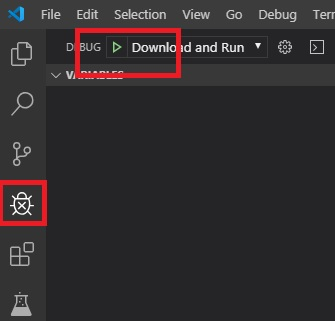
\includegraphics[width=0.5\textwidth]{run.jpg}
              \caption{Configuration}
            \end{center}
        \end{figure}
    

\end{enumerate}


\end{document}
